\section*{Template}


% following notes can be excluded for the actual documentation
\textit{Guidelines:} Die Ergebnisse des Weihnachtsprojekts sollten mit Hilfe der vorgegebenen Vorlage  visualisiert und diskutiert werden. 
Der Bericht sollte dabei eine maximale Länge von acht Seiten nicht überschreiten, die Aufgabenstellung wird hierbei nicht erneut aufgeführt. 
Zur Darstellung und Diskussion können die angehängten Tabellen- und Abbildungsvorlagen verwendet werden, siehe Tab.~\ref{tab:DH} sowie Abb.~\ref{fig:Roboter} und~\ref{fig:plot_example}. 
Etwaige Literatur sollte sauber referenziert werden, z.B. mittels Bibtex~\cite{FehrSchmidSchneiderEberhard20,Fuchs23, DenavitHartenberg55,Lipkin05}.

\textit{Software Guidelines:}
Zusätzlich zur Dokumentation sollen die Simulationsdateien abgegeben werden.
Es ist auf eine ausreichende Kommentierung der Skripte und Funktionen zu achten, numerische Parameter sollen mittels eines Initialisierungsskripts eingebunden werden.

\textit{Gruppenarbeit:}
Es bietet sich an Simulations- und Dokumentationsdateien mit Hilfe von Versionskontrolle gemeinsam zu verwalten, beispielsweise durch den Github-Server der Universität Stuttgart, siehe \href{https://www.tik.uni-stuttgart.de/dienste-a-z/Git-Hosting/}{TIK GitHub}.

% actual documentation starting ...
%\setcounter{section}{0}
%\section{Modifizierte DH-Parameter und Vorwärtskinematik}



\clearpage
%\subsection*{Vorlagen}


\begin{figure}[t]
	\centering
	\includegraphics[height=7cm]{img/Versuchsaufbau.png}
	%	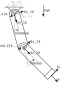
\includegraphics[height=7cm]{img/Zeichnung/Zeichnung.pdf}
	\hspace{1cm}
	\def\svgwidth{5.5cm}
	\input{img/Zeichnung/Zeichnung.pdf_tex}
	\caption{Foto sowie schematische Darstellung des zu untersuchenden Roboters~\cite{Fuchs23}.}
	\label{fig:Roboter}
\end{figure}

\def\myLineWidth{1.5pt}

% may define colors in advance, e.g., if they should be the same throughout the article
\definecolor{mycolor1}{cmyk}{100,70,0,0}%
\definecolor{mycolor2}{RGB}{255, 68, 76}% 
\begin{figure}[t]
	\centering
	% Minimal example for a TikZ plot

% 1) begin the overall picture
\begin{tikzpicture} 
    % 2) begin the axis
    \begin{axis}[%
        % 2a) define the properties of the axis
        width=\textwidth,   % width of the plot
        height= 5cm,       % height of the plot
        xmajorgrids,        % grid on
        xmin = -1,
        xmax = 11,
        ymajorgrids,
        ylabel={Auslenkung $\unit[y]{(m)}$},  % axis label (unit needs units-package)
        xlabel={Zeit $\unit[t]{(s)}$}
        ]
        
        % further may necessary setting:
%        xtick={0.5*pi, pi, 1.5*pi, 2*pi},   % modified xtick positions
%        xticklabels={$\pi/2$,$\pi$,$\nicefrac{3\pi}{2}$,$2\pi$},              % labels at previously set positions
%        ytick={-1,0,1},                 % analogous to x-ticks
%        yticklabels={-$\hat{y}$,0,$\hat{y}$}, 

%        ylabel={displacement $\unit[y]{(m)}$},  % axis label
%        % define legend
%        legend style={
%        	draw=black, % color of the border
%        	at={(0.5,1.05)}, % position plot has normalized wodth and length of 1
%        	anchor = south, % set legend at which anchor to defined position
%        	legend columns = 2, % legend entries in two columns
%        	/tikz/every even column/.append style={column sep=0.5cm} % space between legend's columns
%        }
%        ]
        
        
        % 2b) the plots itselves
        
        % insert data from txt-file
        \addplot[color = mycolor1, line width = \myLineWidth] table{img/plots/data/sin_data.txt}; % define plot properties in [...]
        \addlegendentry{$\sin$} % add legend entry

        \addplot[color = mycolor2, line width = \myLineWidth, dashdotted] table{img/plots/data/cos_data.txt}; % insert data from txt-file
        \addlegendentry{$\cos$} % add legend entry
        
        % manual plot
        \addplot[color = black, line width = 2.0, opacity = 0.5, forget plot] table[row sep=crcr] {%
        	%
        	-5	1\\
        	15 1\\
        }; 
    
    \end{axis}
    
\end{tikzpicture}%

	\caption{Beispielhafter Plot}
	\label{fig:plot_example}
\end{figure}

\bibliographystyle{itm_phd_deu}
\bibliography{literature.bib}
